\documentclass[10pt,a4paper]{article}
\usepackage[utf8]{inputenc}
\usepackage[german]{babel}
\usepackage[T1]{fontenc}
\usepackage{amsmath}
\usepackage{amsfonts}
\usepackage{float}
\usepackage{amssymb}
\usepackage{graphicx}
\renewcommand\thesubsection{\alph{subsection}}
\begin{document}

\begin{center}
\begin{LARGE}
Praktikum 1\\
Differentialgleichungen
\end{LARGE}
\end{center}

\section{Lösung  "`steifer Differentialgleichungen"' mit Euler/Runge-Kutta (RK 2. Ordng.)}

\subsection{Geben Sie das Analogrechner-/Simulink-Schaltbild an.}
\begin{figure}[h]
\centering
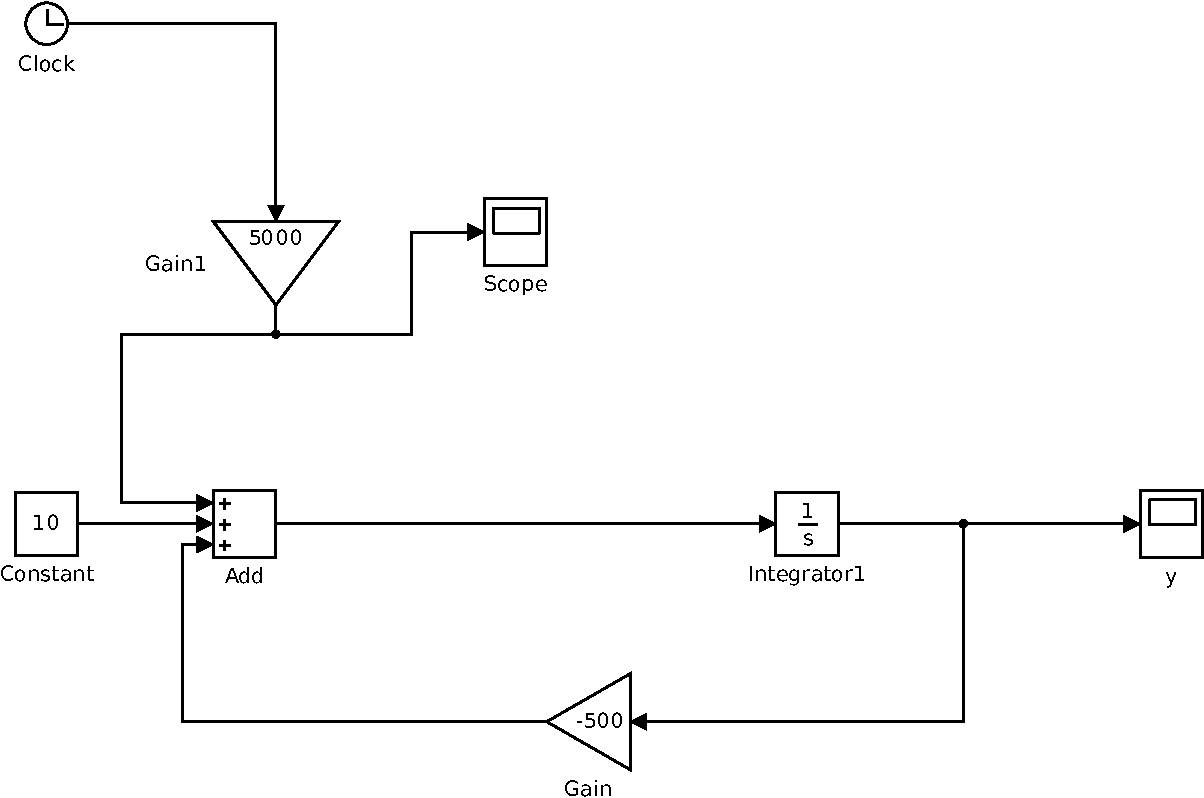
\includegraphics[width=0.9\linewidth]{../screenshots/1}
\end{figure}
\subsection{Geben Sie die Iterationsgleichungen für das Euler-Verfahren an.}
\subsection{Geben Sie die Iterationsgleichungen für das RK2-Verfahren an.}
\subsection{Geben Sie die Iterationsgleichungen für das implizite Euler-Verfahren an.}
\subsection{Schreiben Sie ein Programm "`Stiff.ch"', welches die DGL mit allen Verfahren
löst und zusammen mit der analytischen Lösung in einem Plot anzeigt.}

\begin{center}
\begin{large}
Versuchsdurchführung
\end{large}
\end{center}


\section{Lösung einer (nichtlinearen) DGL 2. Ordnung (Van-der-Pol-DGL) mit RK 2}
\subsection{Geben Sie das Analogrechner-/Simulink-Schaltbild an.}
\begin{figure}[H]
\centering
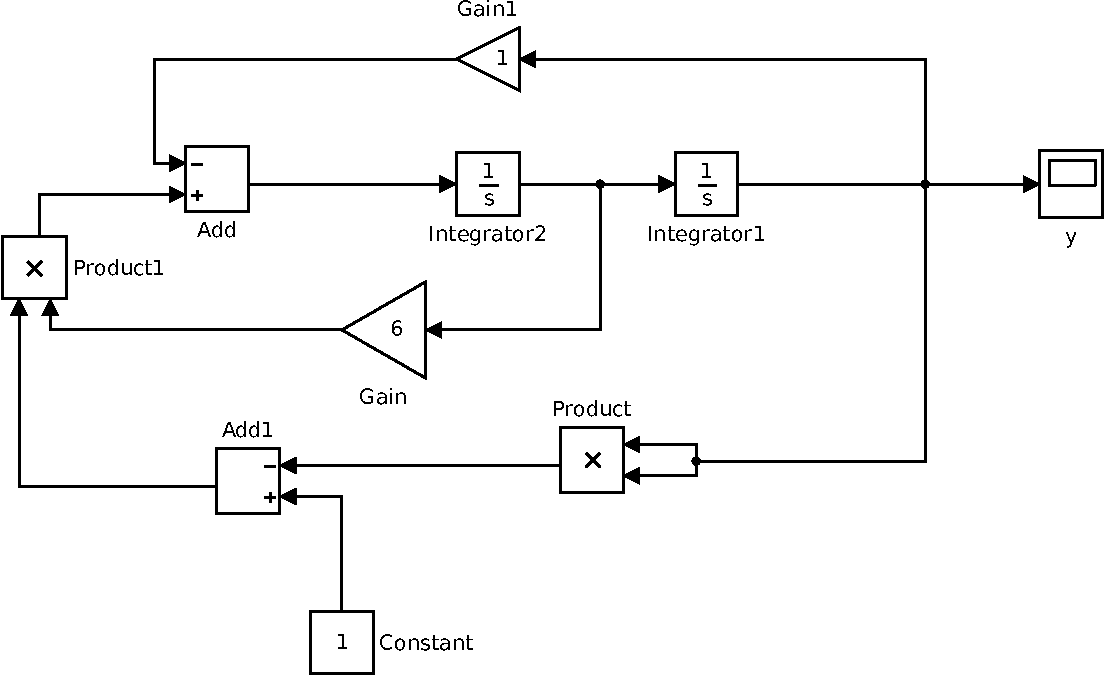
\includegraphics[width=0.9\linewidth]{../screenshots/2}
\end{figure}


\subsection{Geben Sie die DGL 2. Ordnung als 2 DGLn 1. Ordnung an.}

Zerlegung der DGL $y'$ in $y1'$ und $y2'$:
\begin{align}
y'' = 6 * (1-y^2) * y' - y
\\y1' = 6 * (1-y2^2) * y1 - y2
\\y2' = y1
\end{align}

\subsection{Geben Sie die Iterationsgleichungen für das Euler-Verfahren an.}

\begin{align}
y1_{n+1} = y1_n + h * y1'(y1_n,y2_n)
\\y2_{n+1} = y2_n + h * y2'(y2_n)
\\x_{n+1} = x_n + h
\end{align}

\subsection{Geben Sie die Iterationsgleichungen für das RK2-Verfahren an.}

\begin{align}
k1 = h * y1'(y1_n, y2_n);
\\l1 = h * y2'(y1_n);
\\k2 = h * y1'(y1_n + l1/2, y2_n + l1/2);
\\l2 = h * y2'(y1_n + k1/2);
\\y1_{n+1} = y1_n + k2
\\y2_{n+1} = y2_n + l2
\\x_{n+1} = x_n + h
\end{align}

\subsection{Schreiben Sie ein Programm "VanDerPol.ch", welches die DGL mit beiden
Verfahren löst und in einem Plot anzeigt.}

Siehe VanDerPol.ch.

\section{Lösung eines Differentialgleichungssystems (Lorenz-Attraktor) mit RK 2}
\subsection{Geben Sie die Iterationsgleichungen für das RK2-Verfahren an.}
\subsection{Schreiben Sie ein Programm "Lorenz.ch", welches das DGL-System löst.
Geben Sie im 1. Plot die Funktion x(t) aus:
Geben Sie im 2. Plot z(x) aus.}

Der Plot zeigt bei einer Schrittweite von $h = 0.001$ bei Euler und RK eine sehr genaue Darstellung.

\begin{figure}[h]
\centering
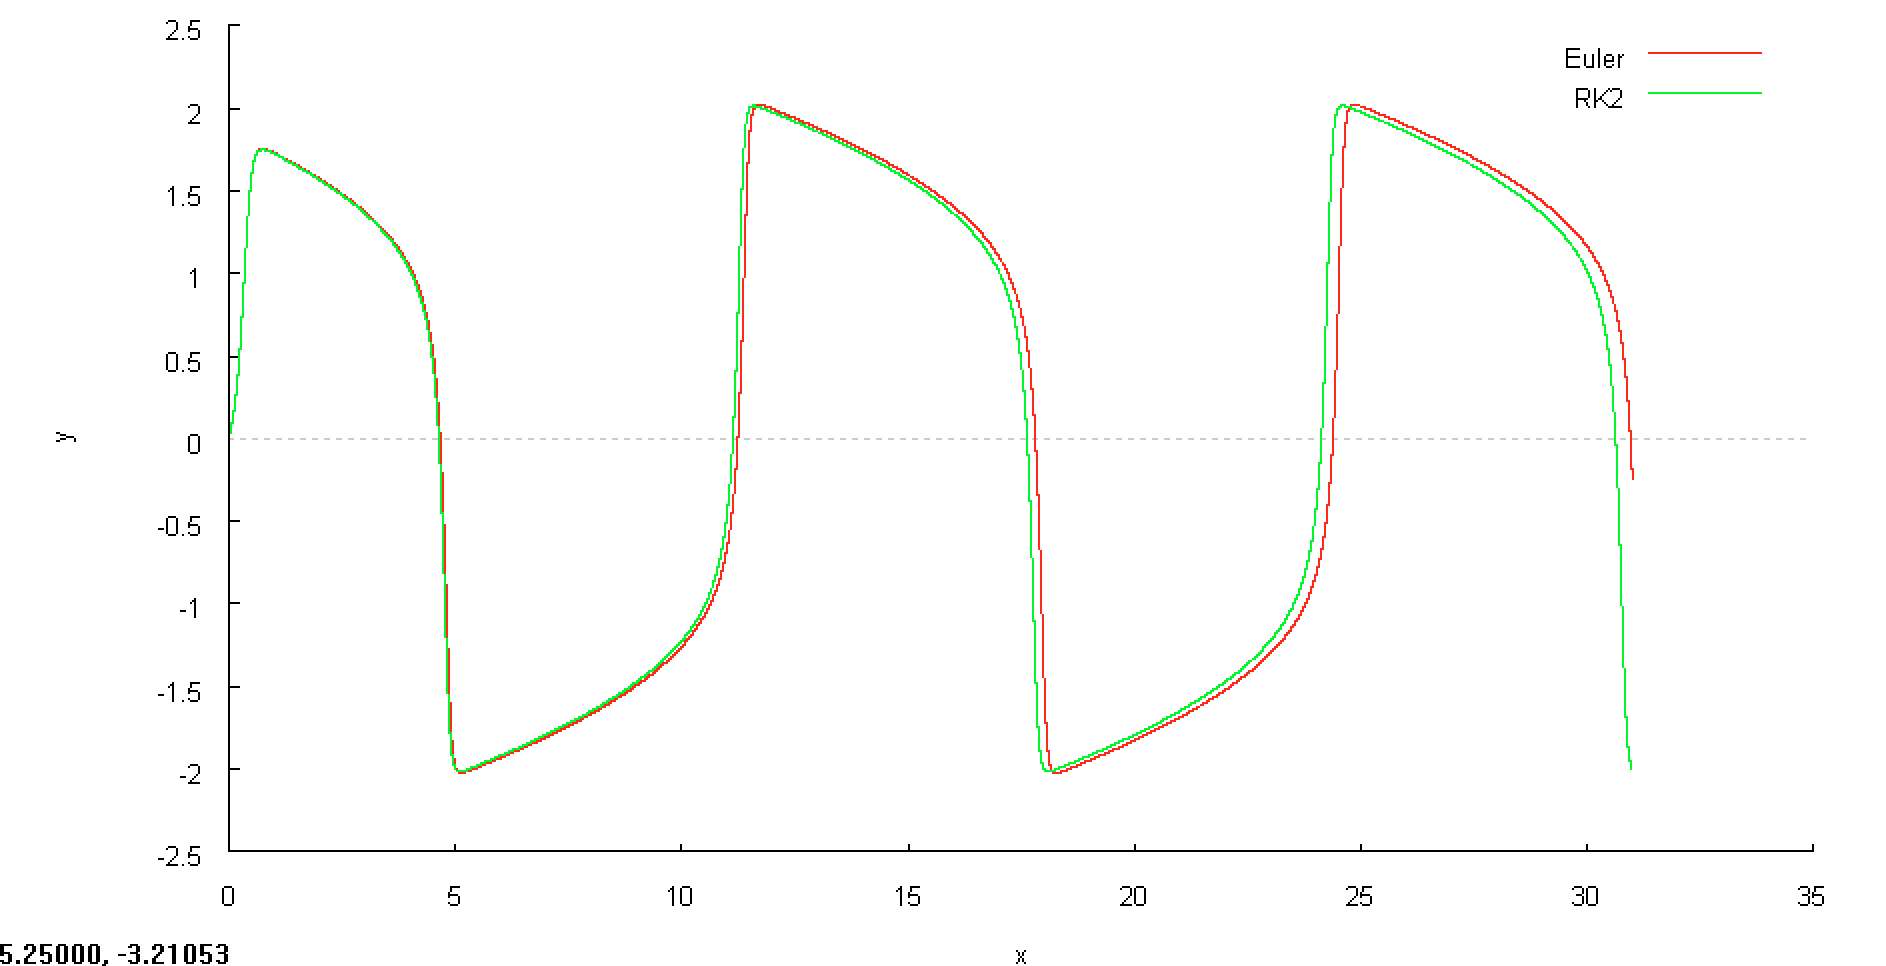
\includegraphics[width=0.9\linewidth]{../screenshots/van001.png}
\end{figure}
Bei einer Schrittweite von $h = 0.2$ sind Euler und RK sehr ungenau, wobei RK noch etwas näher an der korrekten Darstellung ist.
\begin{figure}[h]
\centering
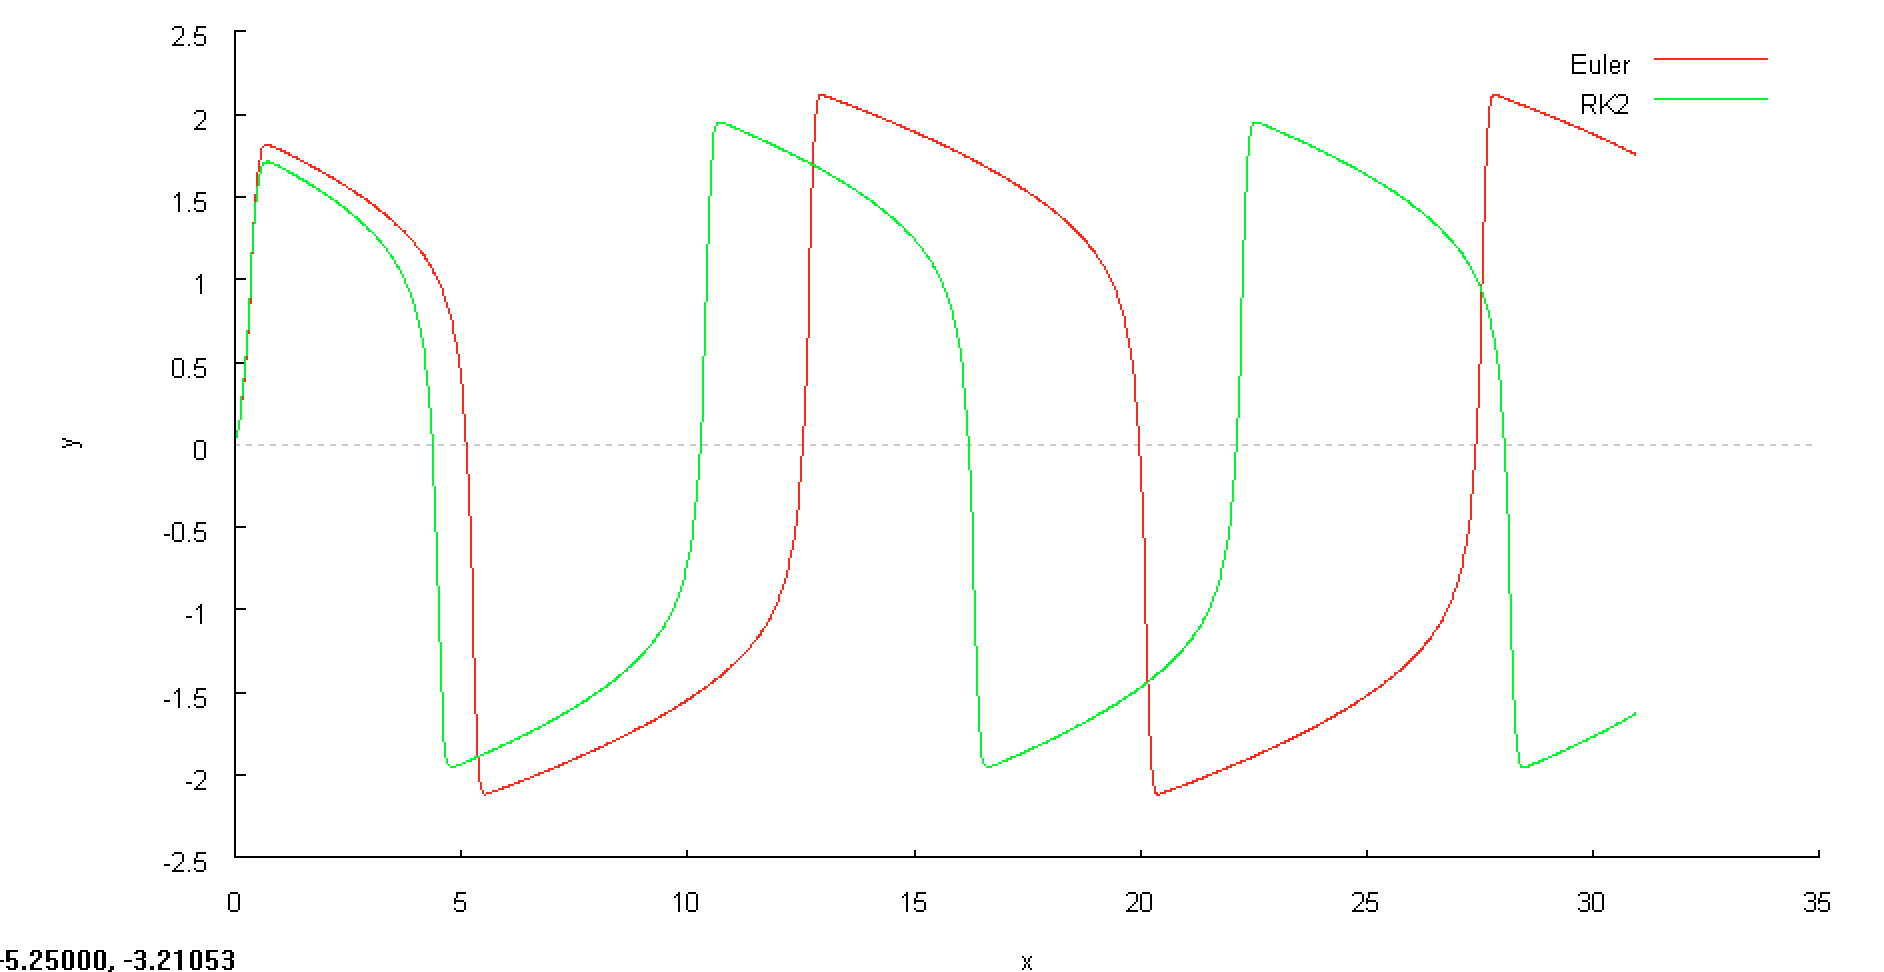
\includegraphics[width=0.9\linewidth]{../screenshots/van02.png}
\end{figure}

\subsection{Realisieren Sie das Differentialgleichungssystem mit MATLab/Simulink}
\begin{figure}[h]
\centering
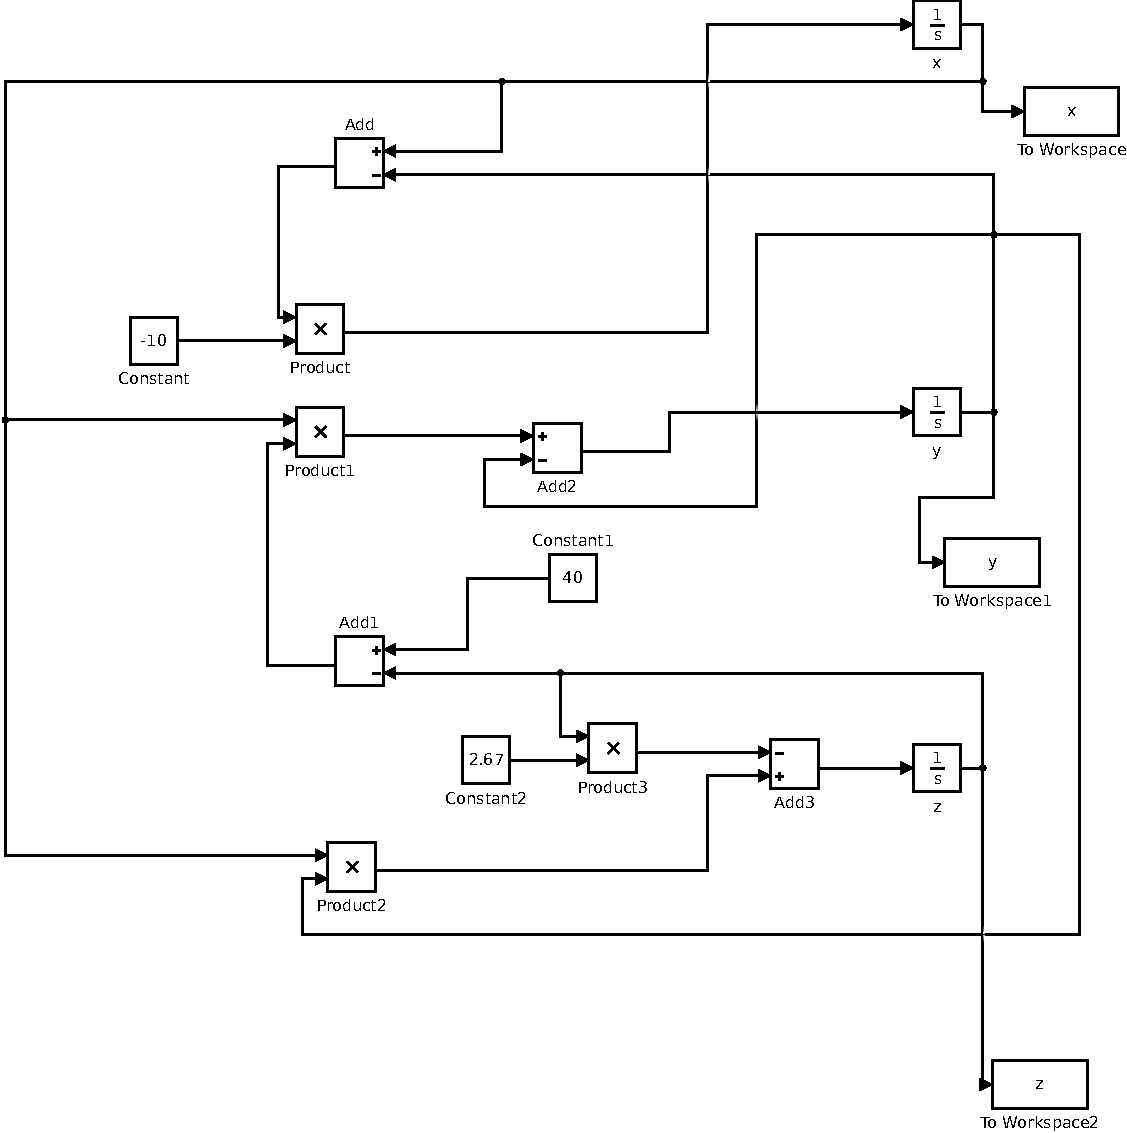
\includegraphics[width=0.9\linewidth]{../screenshots/3}
\end{figure}

\begin{center}
\begin{large}
Versuchsdurchführung
\end{large}
\end{center}

\end{document}